\documentclass{article}
\usepackage{graphicx}
\graphicspath{ {images/} }

\setlength\parindent{0pt}

\begin{document}

FreeRTOS emulator for linux is used on my local machine. Below is a screenshot taken when running the executable.
\newline
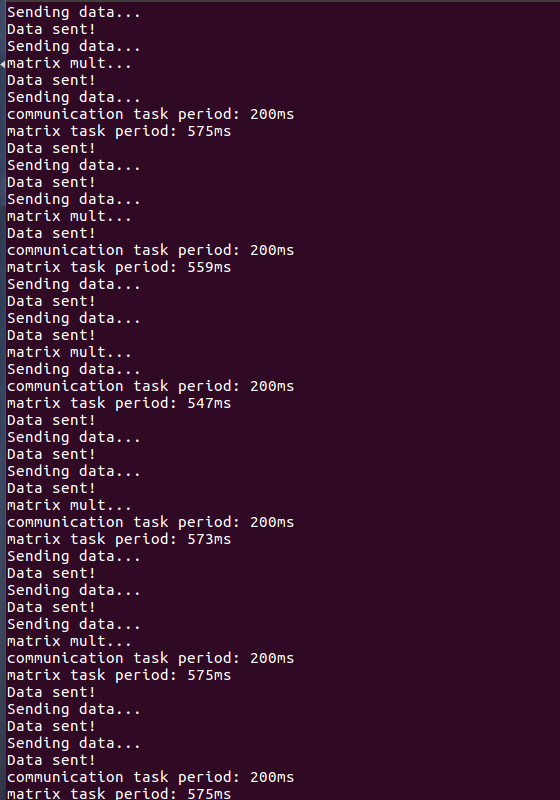
\includegraphics[width=1\textwidth,natwidth=560,natheight=800]{priority_raised.png}
\newline

\newpage

Why is "matrixtask" using most of the CPU utilization?
\newline
Due to a combination of time dependency of long task data/runtime and task's relative high priority, the  matrixtask uses relatively high CPU utilization.
\newline
\newline
Why must the priority of "communicationtask" increase in order for it to work properly?
\newline
The priority must be increased in this case because the underlying RTOS uses priority based task scheduler to divide CPU time to multiple tasks.
\newline
\newline
What happens to the completion time of "matrixtask" when the priority of "communicationtask" is increased?
\newline
The completion time of matrixtask is increased since the scheduler allocates more CPU time to the communicationtask by giving up CPU time from matrixtask. The relative amount of increase depends on the tasks that have their priorities changed higher than the matrixtask's priority.
\newline
\newline
How many seconds is the period of "matrixtask"? (Hint: look at vApplicationTickHook() to measure it)
\newline
The measured period is around 0.570s.

\end{document}
